\section*{Dati e risultati}

Per ogni resistenza a nostra disposizione abbiamo effettuato una misura volt-amperometrica con entrambi i circuiti realizzati. Pertanto per ognuna delle resistenze abbiamo due coppie di valori di corrente e tensione $(I\ped{x}, V\ped{x})$.
In prima approssimazione abbiamo dato una stima del valore delle resistenze sfruttando la legge di Ohm, dal momento che queste sono componenti circuitali Ohmici, e abbiamo ottenuto la seguente relazione: 

\begin{equation}
	R\ped{x} \,=\, \frac{V}{I}
\end{equation}
%
nella quale abbiamo inserito i valori di tensione $(V)$ e di intensità di corrente $(I)$ per ricavare la resistenza incognita $(R\ped{x})$. Facciamo notare che questa stima è grossolana in quanto i valori ricavati non tengono conto della presenza di resistenze interne agli strumenti utilizzati, che possono non essere trascurabili.

Per questo motivo, successivamente, abbiamo calcolato i valori di resistenze risolvendo i due circuiti a nostra disposizione e sfruttando, anche in questo caso la legge integrale di Ohm, abbiamo ottenuto le seguenti relazioni:

\begin{equation}
	\text{Amperomero a monte:} \qquad R\ped{x} \,=\, \frac{V\,R\ped{v}}{R\ped{v}\,I\,-\,V}
\end{equation}
\begin{equation}
	\text{Amperomero a valle:} \qquad R\ped{x} \,=\, \frac{V\,-\,I\,R\ped{a}}{I}
\end{equation}
%
dove $R\ped{x}$ indica il valore della resistenza da stimare, $V$ è la differenza di potenziale misurata con il voltometro, $R\ped{v}$ è la resistenza interna del voltometro, $R\ped{a}$ è la resistenza interna dell'amperometro e $I$ è il valore di corrente misurato grazie all'amperometro.

Inoltre per avere un riscontro che i dati ottenuti siano affidabili abbiamo misurato il valore delle varie resistenze mediante il multimetro digitale. In questo modo potremo osservare se ci sono delle discrepanze rilevanti tra il valore teorico e quello sperimentale delle resistenze. Di seguito è riportato un grafico che metterà a confronto i valori delle resistenze trovati senza risolvere i circuiti e i valori trovati grazie al multimetro.

\begin{SCfigure}[0.6][hbtp]
        \centering
        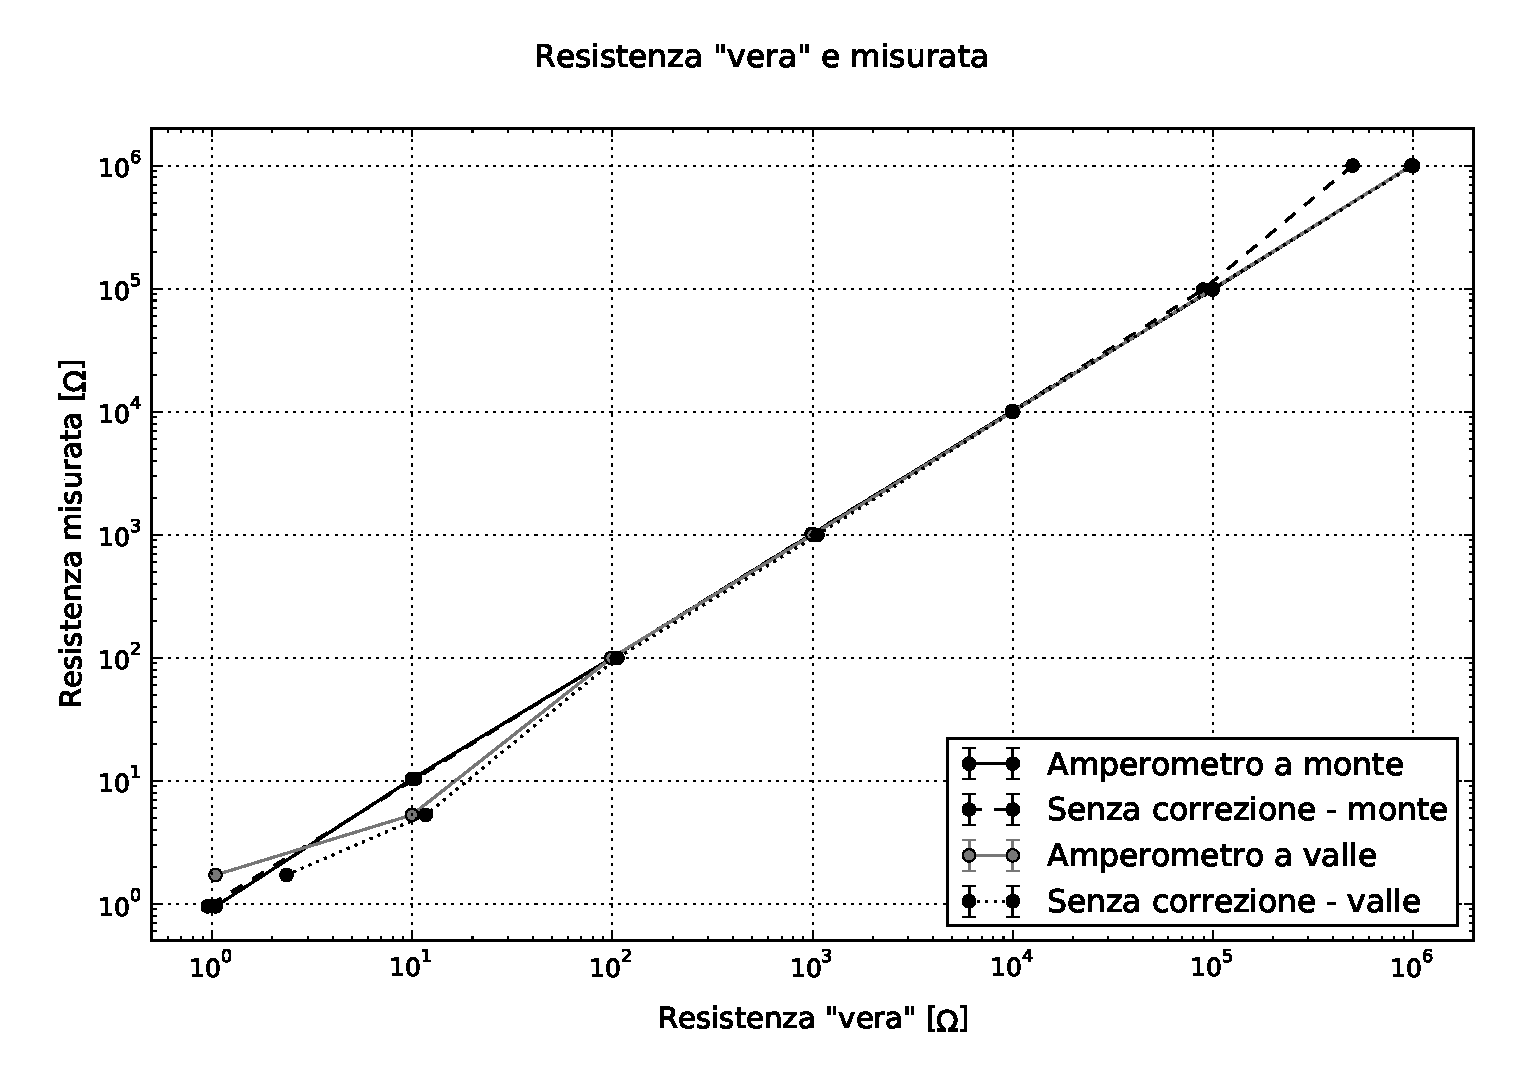
\includegraphics[scale=0.50]{culo.pdf}
        \caption{In questo grafico sono messi a confronto i valori di resistenza misurati mediante il multimetro, che sono riportati sull'asse delle ascisse, e i valori ricavati sfruttando la semplice relazione $R\ped{x} \,=\, \frac{V}{I}$ che si ricava dalla legge di Ohm, valida solo per componenti circuitali Ohmici, che sono riportati sull'asse delle ordinate. Gli errori sulle misure non sono visibili in quanto troppo piccoli rispetto alla scala utilzzata, che ricordiamo essere logaritmica. Inoltre si può notare che la cofigurazione con amperometro a monte è imprecisa per misure di resistenze grandi.}
        \label{fig:culo}
\end{SCfigure}

Infine abbiamo misurato il valore della resistenza di una lampadina, in grado di sopportate una differenza di potenziale massima di $12\,\si{\volt}$, prendendo una serie di misure volt-amperometriche utilizzando entrambi i circuiti a nostra disposizione.
Anche in questo caso abbiamo graficato i dati e abbiamo ottenuto il seguente risultato:

\begin{SCfigure}[0.6][hbtp]
        \centering
        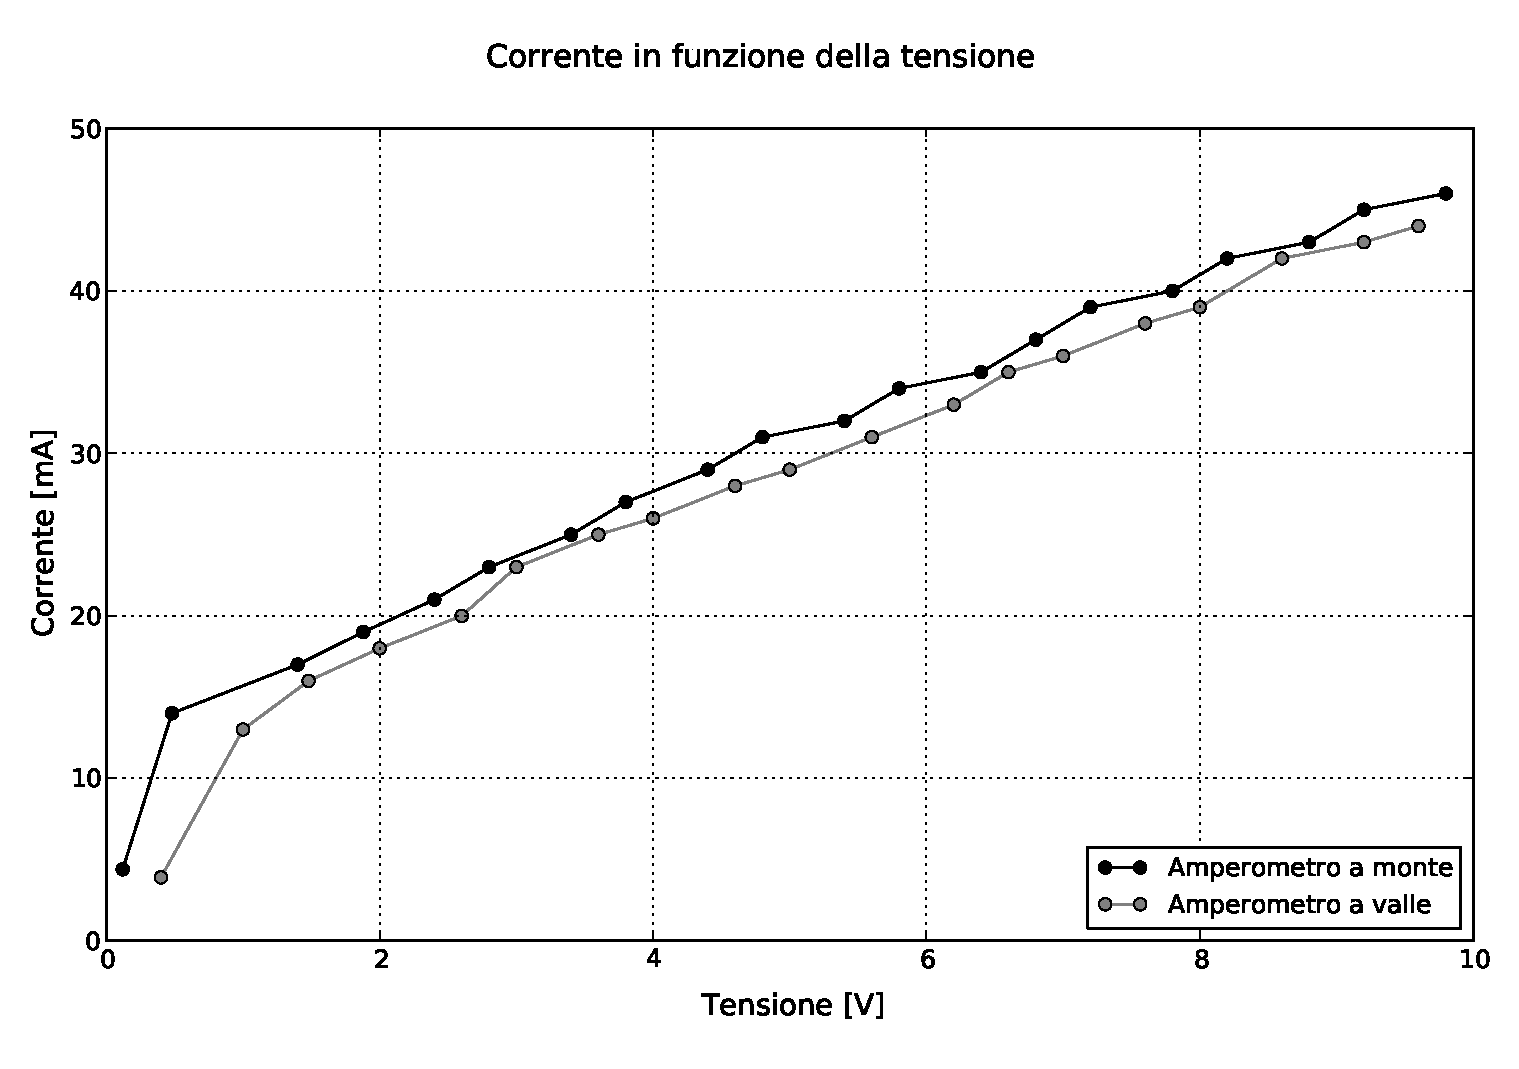
\includegraphics[scale=0.50]{lampadina.pdf}
        \caption{Questo grafico illustra la relazione che sussiste tra la corrente che attraversa la lampadina e la differenza di potenziale ai capi della resistenza interna della stessa. I due set di misure fanno riferimento ai due circuiti utilizzati per acquisire i valori graficati. Le incertezze sui dati non sono visibili in quanto molto piccole rispetto alle scale utilizzate. Come si può notare l'andamento non è lineare, soprattutto per valori piccoli di tensione, questo è giustificato dal fatto che la resistenza della lampadina non è un elemento circuitale Ohmico.}
        \label{fig:lampadina}
\end{SCfigure}

